\chapter{Laufzeitsicht}
Ein wesentlicher Ablauf innerhalb des Matchpunktezählers bildet die Verarbeitung einer eingehenden Bluetooth-Nachricht bis zur Aktualisierung des Frontends. Die Abbildung \ref{fig:sequenzdiagramm}  zeigt ein Sequenzdiagramm in dem dieser Ablauf dargestellt wird.  \\   \\
\begin{minipage}{\textwidth} 
	\centering
	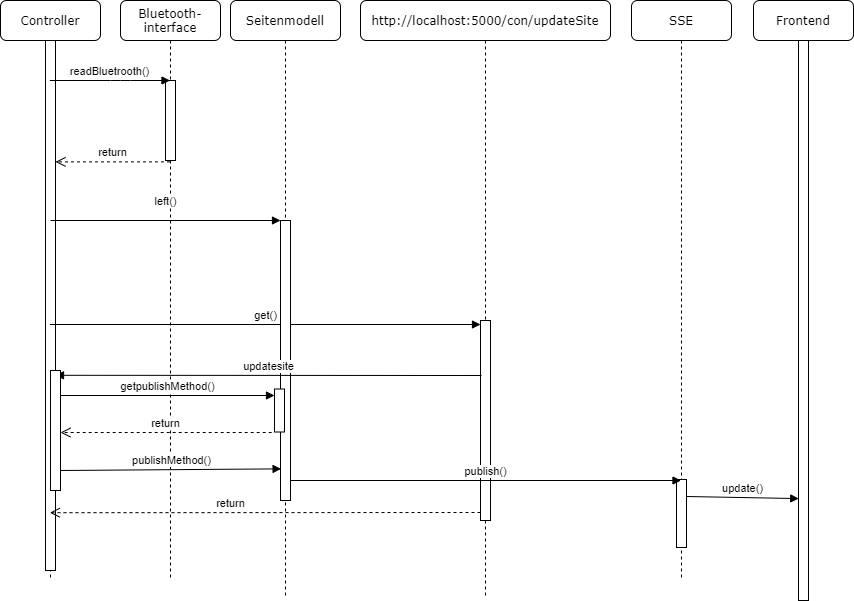
\includegraphics[width=\textwidth]{Bilder/Sequenzdiagramm.png}\\
	\captionof{figure}{Sequenzdiagramm-Diagramm}
	\label{fig:sequenzdiagramm}
\end{minipage}
\\
Der Controller fragt das Bluetooth-Interface in einer Schleife auf Nachrichten vom Bluetooth-Eingabegeräten ab. Wurde eine Nachricht durch einen Tastendruck erkannt, wird die entsprechende Funktion des Seitenmodells aufgerufen. Das Seitenmodell entscheidet, was durch die gedrückte Taste passieren soll.\\   
Außerdem wird über eine HTTP-Verbindung der die Funktion get() des Gunicorn-Servers aufgerufen. Von Dort wird die Funktion updateSide() des des Controllers aufgerufen. Diese Funktion holt sich die publishMethod vom Seitenmodel und ruft diese danach auf.\\
Durch diese wird dann die Funktion publish() aus der SSE-library aufgerufen. Diese sorgt dafür, dass alle Frontends ,die die Events abonniert haben, aktualisiert werden.    